\chapter{مخططات إلينغهام والتعدين}\label{ch:b2:ellingham}

يحوّل الفرن العالي صخرًا أحمر إلى حديد سائل بفحم الكوك والهواء الساخن،
بمعدل آلاف الأطنان في اليوم. ولن يصنع فرن من هذا النوع أبدًا
الألومنيوم ولا المغنيسيوم ولا التيتانيوم، مع أن الكربون رخيص لها بالقدر نفسه.
فأغلب الفلزات توجد في الأرض أكاسيد، واستخلاص فلز يعني
نزع أكسجينه: أي المختزلات تستطيع ذلك، وعند أي
درجة حرارة، مسألةٌ تجيب عنها طاقات جيبس القياسية. وفي سنة 1944 رسمها هارولد
إلينغهام جميعًا على مخطط واحد، بدلالة درجة الحرارة، لمول واحد من ثنائي
الأكسجين في كل منها. فيجيب المخطط بنظرة واحدة: أي فلز يختزل أي أكسيد،
ولماذا يتفوق الكربون عند درجة حرارة مرتفعة، ولماذا يجب صنع بعض الفلزات
بالتحليل الكهربائي.

\begin{recall}
\Cref{ch:b2:reaction-free-energy}: $\Delta_r G^\circ = \Delta_r H^\circ -
T\Delta_r S^\circ$ \omterm{def:b2:reaction-free-energy:ellingham-approximation}{وتقريب إلينغهام} (مستقيمات بدلالة $T$،
باستثناء تغيرات الحالة). \Cref{ch:b2:equilibrium-shifts}: $K^\circ$ انطلاقًا من
$\Delta_r G^\circ$، \omterm{def:b2:equilibrium-shifts:variance}{والتغايرية}، ونهاية التوازن حين يختفي طور.
ومجلد السنة الأولى: أعداد الأكسدة، ومزدوجات الأكسدة والاختزال، والأكاسيد القاعدية
والحمضية. والمجلد المدرسي: الخامات.
\end{recall}

\begin{omfigure}
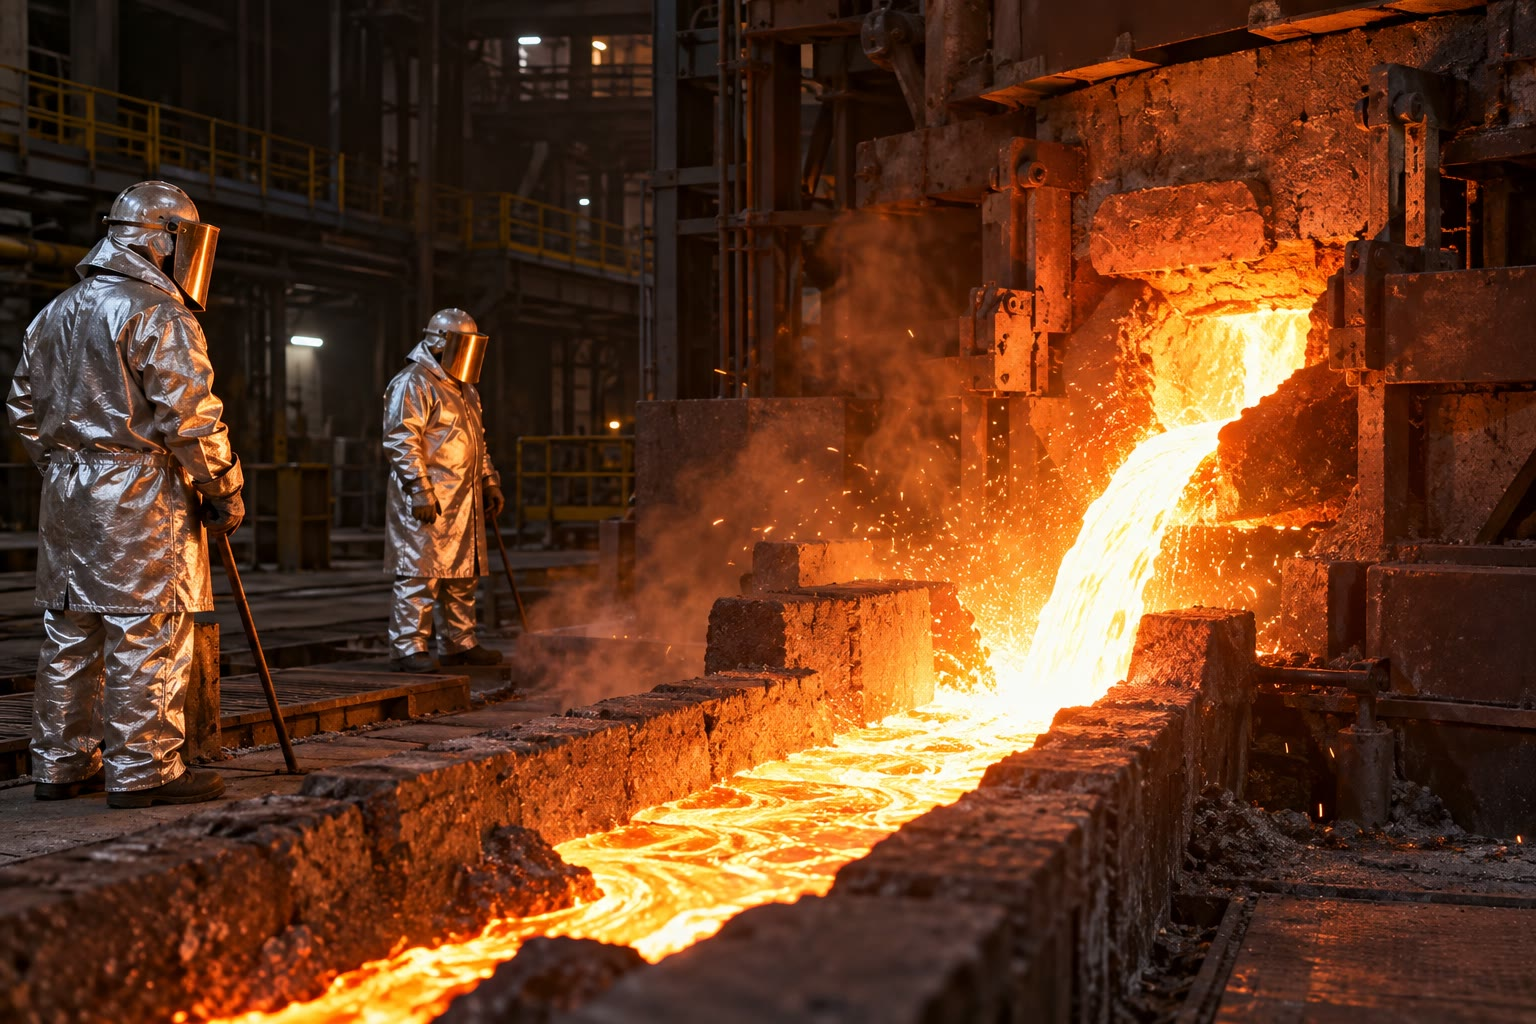
\includegraphics[width=0.62\linewidth]{images/book3/ai/b2-06-blast-furnace.jpg}

{\small فتح ثقب الفرن العالي: يجري الحديد السائل في قناة حرارية، يراقبه
عمال في بزات عاكسة للحرارة. ودرجة الحرارة والغاز
داخل الفرن هما ما يسمح لأحادي أكسيد الكربون بنزع الأكسجين
من أكسيد الحديد.}
\end{omfigure}

\section{مخطط إلينغهام}

لمقارنة ألفة الفلزات المختلفة للأكسجين، تُكتب التفاعلات بحيث
تستهلك كلها الكمية نفسها من الكاشف المشترك.

\begin{definition}[مخطط إلينغهام]\label{def:b2:ellingham:diagram}
\emph{مخطط إلينغهام}\index{مخطط إلينغهام} لعائلة من الأكاسيد
هو المنحنى البياني، بدلالة درجة الحرارة، لطاقات جيبس القياسية لتفاعلات
تكوينها مكتوبةً لمول واحد من ثنائي الأكسجين،
\[
  \tfrac{2x}{y}\,\mathrm M + \ce{O2} \longrightarrow \tfrac{2}{y}\,\mathrm{M}_x\mathrm O_y ,
  \qquad \Delta_r G^\circ(T) \ \text{لكل مول من } \ce{O2} .
\]
\end{definition}

مثل \ce{2Zn + O2 -> 2ZnO}، و\ce{4/3Al + O2 -> 2/3Al2O3}، و\ce{2C + O2 ->
2CO}. والإحداثي العمودي بوحدة \unit{kJ} لكل مول من \ce{O2}، وهو سالب دائمًا
لفلزات المخطط.

\begin{proposition}[المستقيمات]\label{prop:b2:ellingham:line}
في \omterm{def:b2:reaction-free-energy:ellingham-approximation}{تقريب إلينغهام}، كل خط مستقيم، ميله $-\Delta_r
S^\circ$. ومن أجل فلز وأكسيده، وكلاهما مكثف، يكون $\Delta_r S^\circ$
قريبًا من سالب إنتروبيا مول ثنائي الأكسجين المستهلَك، أي نحو
$-\qty{200}{J/(K.mol)}$: فالمستقيمات تصعد مع درجة الحرارة، وكلها تقريبًا
بالميل نفسه.
\end{proposition}

\begin{proof}
$\Delta_r G^\circ = \Delta_r H^\circ - T\Delta_r S^\circ$ مع $\Delta_r
H^\circ$ و$\Delta_r S^\circ$ ثابتين. والإنتروبيات المولية للأجسام الصلبة عشرات من
\unit{J/(K.mol)} وتكاد تُختصر بين الفلز والأكسيد، في حين يُستهلك مول واحد من
الغاز، إنتروبياه $S^\circ(\ce{O2}) = \qty{205}{J/(K.mol)}$. ومن أجل الزنك،
$2(43.65) - 2(41.63) - 205.15 = \qty{-201.1}{J/(K.mol)}$.
% ledger: s0:ZnO_cr, s0:Zn_cr, s0:O2_g
\end{proof}

\begin{proposition}[انكسارات المستقيمات]\label{prop:b2:ellingham:break}
عند درجة الحرارة التي ينصهر فيها الفلز أو يغلي، يتغير ميل الخط:
فيزداد ميله بمقدار $\nu\,\Delta_{\text{تحول}}S$، حيث $\nu$ كمية
الفلز في التفاعل و$\Delta_{\text{تحول}}S = \Delta_{\text{تحول}}H/T_{\text{تحول}}$.
أما تغيّر حالة الأكسيد فيخفض الميل.
\end{proposition}

\begin{proof}
فوق التحوّل يتفاعل الفلز انطلاقًا من طوره الجديد، الذي تكون إنتروبياه
أعلى بمقدار $\Delta_{\text{تحول}}S$: فينخفض $\Delta_r S^\circ$ بمقدار $\nu\,\Delta_{\text{تحول}}S$
ويزداد الميل $-\Delta_r S^\circ$ بالقدر نفسه. أما $\Delta_r G^\circ$
نفسه فمتصل، لأن للطورين عند $T_{\text{تحول}}$ \omterm{def:b2:chemical-potential:chemical-potential}{الجهد الكيميائي}
نفسه. ومن أجل الأكسيد، الإشارة المعاكسة.
\end{proof}

يغيّر الانصهار الميل قليلًا؛ أما الغليان، الذي يحوّل متفاعلًا مكثفًا
إلى غاز، فيغيّره كثيرًا. يغلي الزنك عند \qty{1180}{K}: فوق هذه
الدرجة يستهلك تكوين أكسيد الزنك ثلاثة مولات من الغاز لكل مولين من
الأكسيد، ويصعد خطه بحدة. ويحدث الشيء نفسه للمغنيسيوم فوق
نقطة غليانه.

\begin{omfigure}
\begin{tikzpicture}[lab/.style={anchor=west, font=\scriptsize, inner sep=1pt}]
\begin{axis}[omellingham,
  width=0.84\linewidth, height=11cm, xmin=300, xmax=2100, ymin=-1250, ymax=0,
  clip mode=individual,
  xlabel={\babelsublr{$T$ (K)}}, ylabel={\foreignlanguage{arabic}{$\Delta_r G^\circ$ بوحدة \unit{kJ} لكل مول من \ce{O2}}},
  xtick={300,500,700,900,1100,1300,1500,1700,1900,2100},
  x tick label style={rotate=45, anchor=north east, font=\scriptsize}]
\addplot[black!60, thick] table[x=T, y=G] {figdata/out/bachelor-2-ellingham-a-HgO.dat};
\addplot[omProp, thick] table[x=T, y=G] {figdata/out/bachelor-2-ellingham-a-Cu2O.dat};
\addplot[omDef, thick] table[x=T, y=G] {figdata/out/bachelor-2-ellingham-a-FeO.dat};
\addplot[omExo, very thick] table[x=T, y=G] {figdata/out/bachelor-2-ellingham-a-ZnO.dat};
\addplot[black!60, thick] table[x=T, y=G] {figdata/out/bachelor-2-ellingham-a-Cr2O3.dat};
\addplot[omProp, thick] table[x=T, y=G] {figdata/out/bachelor-2-ellingham-a-TiO2.dat};
\addplot[omDef, thick] table[x=T, y=G] {figdata/out/bachelor-2-ellingham-a-Al2O3.dat};
\addplot[black!60, thick] table[x=T, y=G] {figdata/out/bachelor-2-ellingham-a-MgO.dat};
\addplot[omProp, thick] table[x=T, y=G] {figdata/out/bachelor-2-ellingham-a-CaO.dat};
\addplot[omThm, very thick] table[x=T, y=G] {figdata/out/bachelor-2-ellingham-a-C-CO.dat};
\addplot[omThm, thick, dashed] table[x=T, y=G] {figdata/out/bachelor-2-ellingham-a-C-CO2.dat};
\addplot[omThm, thick, dotted] table[x=T, y=G] {figdata/out/bachelor-2-ellingham-a-CO-CO2.dat};
\addplot[omDef, thick, dashed] table[x=T, y=G] {figdata/out/bachelor-2-ellingham-a-H2-H2O.dat};
% labels: inside for the two short lines, at the right end for the others
\node[font=\scriptsize, black!70, anchor=south] at (axis cs:400,-60) {\ce{HgO}};
\node[font=\scriptsize, omProp, anchor=south] at (axis cs:1100,-150) {\ce{Cu2O}};
\draw[omExo, thin] (axis cs:2100,-69) -- (axis cs:2150,-60) node[lab, text=omExo] {\ce{ZnO}};
\draw[omThm, thin] (axis cs:2100,-204) -- (axis cs:2150,-185) node[lab, text=omThm] {$\ce{CO}/\ce{CO2}$};
\draw[omDef, thin] (axis cs:2100,-259) -- (axis cs:2150,-235) node[lab, text=omDef] {$\ce{H2}/\ce{H2O}$};
\draw[omDef, thin] (axis cs:2100,-286) -- (axis cs:2150,-285) node[lab, text=omDef] {\ce{FeO}};
\draw[black!70, thin] (axis cs:2100,-393) -- (axis cs:2150,-365) node[lab, text=black!70] {\ce{Cr2O3}};
\draw[omThm, thin] (axis cs:2100,-396) -- (axis cs:2150,-415) node[lab, text=omThm] {$\ce{C}/\ce{CO2}$};
\draw[omProp, thin] (axis cs:2100,-567) -- (axis cs:2150,-540) node[lab, text=omProp] {\ce{TiO2}};
\draw[omThm, thin] (axis cs:2100,-589) -- (axis cs:2150,-590) node[lab, text=omThm] {$\ce{C}/\ce{CO}$};
\draw[black!70, thin] (axis cs:2100,-600) -- (axis cs:2150,-640) node[lab, text=black!70] {\ce{MgO}};
\draw[omDef, thin] (axis cs:2100,-668) -- (axis cs:2150,-690) node[lab, text=omDef] {\ce{Al2O3}};
\draw[omProp, thin] (axis cs:2100,-765) -- (axis cs:2150,-765) node[lab, text=omProp] {\ce{CaO}};
\end{axis}
\end{tikzpicture}

{\small \omterm{def:b2:ellingham:diagram}{مخطط إلينغهام}: \omterm{def:b2:reaction-free-energy:reaction-gibbs}{طاقة جيبس القياسية} لتكوين الأكاسيد
لكل مول من \ce{O2}، بدلالة درجة الحرارة، من طاقات جيبس المجدولة. وكلما
انخفض خط كان الأكسيد أكثر استقرارًا والفلز أشد اختزالًا.
وكل خط فلز موسوم بأكسيده؛ و$\ce{C}/\ce{CO}$ هو \ce{2C + O2 -> 2CO}،
و$\ce{C}/\ce{CO2}$ هو \ce{C + O2 -> CO2}، و$\ce{CO}/\ce{CO2}$ هو \ce{2CO + O2 -> 2CO2}،
و$\ce{H2}/\ce{H2O}$ هو \ce{2H2 + O2 -> 2H2O}، والماء غاز.}
% ledger: janafG:Cu2O.300, janafG:FeO.300, janafG:Cr2O3.300, janafG:TiO2.500, janafG:Al2O3.300, janafG:MgO.300, janafG:CaO.300, janafG:CO.300, janafG:CO2.300, janafG:H2O.300, dfh:ZnO_cr, dfh:HgO_cr, s0:HgO_cr, s0:Hg_l, s0:Hg_g, dfh:Hg_g (all temperatures in figdata/bachelor-2/ellingham.py)
\end{omfigure}

\section{قراءة المخطط}

\begin{definition}[ضغط الأكسجين التوازني]\label{def:b2:ellingham:oxygen-pressure}
\emph{ضغط الأكسجين التوازني}\index{ضغط الأكسجين التوازني} لزوج
فلز--أكسيد عند درجة الحرارة $T$ هو ضغط ثنائي الأكسجين الذي يتعايش عنده الفلز
والأكسيد في توازن: $RT\ln(p_{\ce{O2}}/p^\circ) = \Delta_r
G^\circ(T)$ للتفاعل المكتوب لكل مول من \ce{O2}.
\end{definition}

\begin{theorem}[منطقتا الفلز والأكسيد]\label{thm:b2:ellingham:domains}
في جو ضغط الأكسجين فيه $p_{\ce{O2}}$ عند درجة الحرارة $T$، يتأكسد
الفلز إذا كان $RT\ln(p_{\ce{O2}}/p^\circ) > \Delta_r G^\circ(T)$، ويُختزل
الأكسيد إلى الفلز إذا كان $RT\ln(p_{\ce{O2}}/p^\circ) < \Delta_r
G^\circ(T)$. وعلى المخطط، يكون الأكسيد مستقرًا فوق خطه، والفلز
تحته.
\end{theorem}

\begin{proof}
مع فلز وأكسيد مكثفين نشاطية كل منهما 1، يكون $Q = p^\circ/p_{\ce{O2}}$ 
و$\Delta_r G = \Delta_r G^\circ + RT\ln Q = \Delta_r G^\circ - RT\ln(p_{\ce{O2}}/
p^\circ)$. ويجري التأكسد في الاتجاه المباشر حين $\Delta_r G < 0$.
\end{proof}

في الهواء ($p_{\ce{O2}} = \qty{0.21}{bar}$، و$RT\ln 0.21$ يساوي \qty{-4}{kJ/mol}
في درجة حرارة الغرفة و\qty{-13}{kJ/mol} عند \qty{1000}{K}، أي صفرًا تقريبًا على هذا
السلم) يتأكسد كل فلز في المخطط يقع خطه
تحت المحور: ففي درجة حرارة الغرفة كلها، حتى النحاس.
ولا تتفكك إلا الأكاسيد القريبة من الأعلى (الفضة، الزئبق) بتسخين
معتدل.

\begin{example}[أكسيد الزئبق]\label{ex:b2:ellingham:hgo}
من أجل \ce{2Hg + O2 -> 2HgO}، تعطي قيم كوداتا المرجعية $\Delta_r H^\circ =
\qty{-181.6}{kJ/mol}$ مع الزئبق السائل؛ وفوق نقطة غليان الزئبق
يكون الفلز غازًا و$\Delta_r H^\circ = \qty{-304.3}{kJ/mol}$، و$\Delta_r
S^\circ = \qty{-414.6}{J/(K.mol)}$. ويقطع الخط الصفر عند
$T = 304.3/0.4146 \approx \qty{734}{K}$: فإذا سُخّن أكسيد الزئبق الأحمر فوق هذه الدرجة في الهواء،
أو تحت \qty{1}{bar} من الأكسجين، أطلق أكسجينه ---
وبهذه الطريقة عُزل الأكسجين أول مرة سنة 1774.
% ledger: dfh:HgO_cr, s0:HgO_cr, s0:Hg_l, s0:Hg_g, dfh:Hg_g, s0:O2_g (computed in figdata/bachelor-2/ellingham.py)
\end{example}

\begin{proposition}[أي فلز يختزل أي أكسيد]\label{prop:b2:ellingham:reduction}
عند درجة حرارة معيّنة، يختزل فلز M أكسيدَ فلز N، في
الشروط القياسية، حين يقع خط M تحت خط N. \omterm{def:b2:reaction-free-energy:reaction-gibbs}{وطاقة جيبس القياسية
لتفاعل} الاختزال، لكل مول من \ce{O2} المنقول، هي
فرق الإحداثيين العموديين.
\end{proposition}

\begin{proof}
الاختزال هو تكوين أكسيد M ناقص تكوين أكسيد N، وكلاهما لكل
مول من \ce{O2}: $\Delta_r G^\circ = \Delta_r G^\circ_{\mathrm M} - \Delta_r
G^\circ_{\mathrm N}$، وهو سالب حين يكون خط M أدنى.
\end{proof}

\begin{method}[قراءة مخطط إلينغهام]\label{met:b2:ellingham:read-ellingham}
\begin{enumerate}
  \item جِد الخطين عند درجة الحرارة المعنية. الأدنى منهما هو
        الأكسيد الأكثر استقرارًا؛ وفلزه يختزل الأكسيد الآخر.
  \item الفجوة العمودية هي $\Delta_r G^\circ$ لكل مول من \ce{O2}: فجوة قدرها
        \qty{100}{kJ} أو أكثر تعني اختزالًا تامًا عمليًا.
  \item حيث يتقاطع خطان ينقلب اتجاه الاختزال: اقرأ
        درجة حرارة التقاطع.
  \item انتبه للانكسارات: فالفلز الذي يغلي داخل الفترة يغادر على هيئة
        بخار، يمكن فصله بالتقطير --- أو يعود فيتأكسد عند التبريد.
\end{enumerate}
\end{method}

\begin{definition}[الاختزال الألومنيوحراري]\label{def:b2:ellingham:aluminothermy}
\emph{الاختزال الألومنيوحراري}\index{اختزال ألومنيوحراري} هو
اختزال أكسيد فلزي بمسحوق الألومنيوم، وهو ممكن لكل أكسيد يقع
خطه فوق خط الألومينا، وشديد النشر للحرارة إلى حد انصهار الخليط:
\ce{Fe2O3 + 2Al -> Al2O3 + 2Fe} (الثرميت) يلحم السكك؛ و\ce{Cr2O3 + 2Al ->
Al2O3 + 2Cr} يصنع كرومًا خاليًا من الكربون.
\end{definition}

\begin{omfigure}
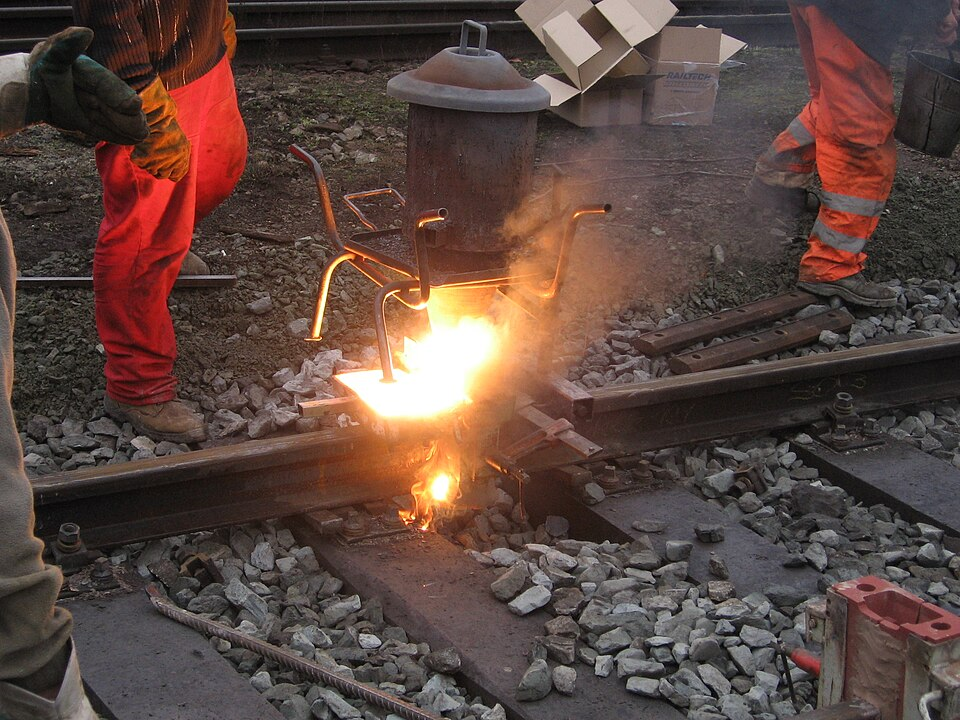
\includegraphics[width=0.5\linewidth]{images/book3/thermite.jpg}

{\small لحام سكة بالثرميت: تفاعل أكسيد الحديد مع الألومنيوم
في البوتقة فوق الوصلة يعطي حديدًا سائلًا، يسيل إلى
القالب بين طرفي السكتين. (صورة: بيترس، CC~BY-SA~3.0، ويكيميديا كومنز.)}
\end{omfigure}

\section{الكربون وأحادي أكسيد الكربون}

ثلاثة خطوط تخص الكربون:
\begin{itemize}
  \item \ce{C + O2 -> CO2}: مول واحد من الغاز يعطي مولًا واحدًا، $\Delta_r S^\circ
        \approx 0$، خط أفقي تقريبًا قرب \qty{-395}{kJ}؛
  \item \ce{2C + O2 -> 2CO}: مول واحد من الغاز يعطي مولين، $\Delta_r S^\circ
        \approx \qty{+180}{J/(K.mol)}$، خط \emph{ينحدر} مع درجة الحرارة؛
  \item \ce{2CO + O2 -> 2CO2}: ثلاثة مولات من الغاز تعطي مولين، خط صاعد.
\end{itemize}

\begin{proposition}[الكربون يختزل كل شيء تقريبًا على الساخن]\label{prop:b2:ellingham:carbon}
ينحدر خط \ce{2C + O2 -> 2CO} مع درجة الحرارة ويقطع
خطوط أغلب الأكاسيد الفلزية: فوق درجة حرارة التقاطع يختزل الكربون
الأكسيد، معطيًا أحادي أكسيد الكربون. ويقع التقاطع مع أكسيد الحديد(II) قرب
\qty{1040}{K}، ومع أكسيد الزنك قرب \qty{1220}{K}؛ ومع أكسيد التيتانيوم وأكسيد المغنيسيوم
قرب \qty{2000}{K} أو فوقها، ومع الألومينا أعلى من ذلك أيضًا، حيث تتحد
الفلزات بالكربون مكوّنة كربيدات أو تعود فتتأكسد مع تبرد الغاز.
\end{proposition}

\begin{proof}
الميل $-\Delta_r S^\circ$ لخط الكربون سالب ($\Delta\nu_{\text{غاز}}
= +1$)، وميل خطوط الأكاسيد موجب: فتلتقي مرة واحدة. ودرجات الحرارة
مقروءة على الخطوط المحسوبة.
% ledger: janafG:CO.900, janafG:CO.1100, janafG:FeO.900, janafG:FeO.1100 (crossings computed in figdata/bachelor-2/ellingham.py)
\end{proof}

\begin{definition}[توازن بودوار]\label{def:b2:ellingham:boudouard}
\emph{توازن بودوار}\index{توازن بودوار} هو \ce{C(s) + CO2(g) <=> 2CO(g)}،
\omterm{def:b2:reaction-enthalpy:exothermic}{الماص للحرارة}، بين الكربون وأكسيدي الكربون.
\end{definition}

\begin{proposition}[تركيب الغاز فوق الكربون]\label{prop:b2:ellingham:boudouard}
\omterm{def:b2:equilibrium-shifts:variance}{تغايرية} النظام كربون + \ce{CO} + \ce{CO2} تساوي 2: فعند $T$ وضغط كلي $p$
معلومين، يتحدد الكسر المولي $x$ لأحادي أكسيد الكربون بالعلاقة $x^2/(1 - x)
= K^\circ(T)\,p^\circ/p$. وعند \qty{1}{bar} يكون الغاز \ce{CO2} شبه نقي
تحت \qty{700}{K} و\ce{CO} شبه نقي فوق \qty{1200}{K}؛ وتقاطع
خطوط الكربون الثلاثة، قرب \qty{975}{K}، هو حيث $K^\circ = 1$.
\end{proposition}

\begin{proof}
ثلاثة أنواع، وتفاعل واحد، وطوران: $v = 3 - 1 + 2 - 2 = 2$. ومع $p_{\ce{CO}}
= xp$ و$p_{\ce{CO2}} = (1 - x)p$، يكون $Q = x^2p/[(1 - x)p^\circ]$. وعند $K^\circ = 1$
تتساوى طاقتا جيبس القياسيتان للتفاعلين \ce{2C + O2 -> 2CO} و\ce{C + O2 -> CO2}:
فيلتقي الخطان، ومن ثم الثالث.
\end{proof}

\begin{omfigure}
\begin{tikzpicture}
\begin{axis}[
  width=0.62\linewidth, height=5.4cm, xmin=500, xmax=1500, ymin=0, ymax=1.05,
  axis x line=bottom, axis y line=left, xlabel={\babelsublr{$T$ (K)}},
  xtick={500,700,900,1100,1300,1500}, ytick={0,0.5,1},
  ylabel={\foreignlanguage{arabic}{الكسر المولي لأحادي أكسيد الكربون \ce{CO}}}, tick label style={font=\small},
  label style={font=\small}, clip=false]
\addplot[omThm, very thick] table[x=T, y=xCO] {figdata/out/bachelor-2-ellingham-b.dat};
\node[font=\scriptsize, anchor=west] at (axis cs:1150,0.55) {\foreignlanguage{arabic}{\ce{CO} مستقر}};
\node[font=\scriptsize, anchor=west] at (axis cs:510,0.6) {\shortstack{\foreignlanguage{arabic}{\ce{CO2} (والكربون) مستقران}}};
\end{axis}
\end{tikzpicture}

{\small \omterm{def:b2:ellingham:boudouard}{توازن بودوار} عند \qty{1}{bar}: الكسر المولي لأحادي أكسيد
الكربون في غاز في توازن مع الكربون.}
% ledger: janafG:CO.700, janafG:CO2.700, janafG:CO.1100, janafG:CO2.1100 (computed in figdata/bachelor-2/ellingham.py)
\end{omfigure}

\section{الفرن العالي}

يُشحن خام الحديد (الهيماتيت \ce{Fe2O3}، والماغنيتيت \ce{Fe3O4}) وفحم الكوك والحجر
الجيري من أعلى عمود طويل؛ ويُنفخ الهواء الساخن
قرب أسفله. وفي هبوطها تلاقي المواد الصلبة غازًا ساخنًا صاعدًا؛ ويغادر الغاز
من الأعلى، وقد برد.
\begin{itemize}
  \item عند المنافخ يحترق فحم الكوك في الهواء الساخن: \ce{C + O2 -> CO2}، 
        وفوق ذلك، مع فائض الكربون، \ce{CO2 + C -> 2CO} (بودوار): فالغاز
        الصاعد أغلبه أحادي أكسيد الكربون والنيتروجين.
  \item في الجزء العلوي، يختزل أحادي أكسيد الكربون أكاسيد الحديد مرحلة
        بعد مرحلة، \ce{3Fe2O3 + CO -> 2Fe3O4 + CO2}، \ce{Fe3O4 + CO -> 3FeO + CO2}،
        \ce{FeO + CO -> Fe + CO2}. والمرحلتان الأوليان سهلتان؛ أما في الأخيرة
        فيمر خط $\ce{CO}/\ce{CO2}$ \textit{فوق} خط
        \ce{FeO} بقليل: \omterm{def:b2:reaction-free-energy:reaction-gibbs}{فطاقة جيبس القياسية لتفاعلها} موجبة بقليل
        ($K^\circ \approx 0.3$ عند \qty{900}{K})، ويتطلب الاختزال غازًا
        فيه من \ce{CO} ثلاثة أضعاف ما فيه من \ce{CO2} على الأقل --- وهو ما
        يوفره \omterm{def:b2:ellingham:boudouard}{توازن بودوار} في المنطقة الساخنة تحته.
  \item في الأسفل، حيث الحرارة أشد، يختزل الكربون نفسه ما تبقى، \ce{FeO + C ->
        Fe + CO}؛ فيذيب الحديد الكربون، وينصهر، ويتجمع في القاع
        مع خبث منصهر يتكوّن من الجير والسيليكا الموجودة في الخام.
\end{itemize}

\begin{omfigure}
\begin{tikzpicture}[font=\small, >={Stealth}]
  \fill[gray!12] (-1.4,0) -- (-2.0,3.0) -- (-1.3,7.0) -- (1.3,7.0) -- (2.0,3.0) -- (1.4,0) -- cycle;
  \draw[thick] (-1.4,0) -- (-2.0,3.0) -- (-1.3,7.0) (1.4,0) -- (2.0,3.0) -- (1.3,7.0);
  \draw[thick] (-1.4,0) -- (1.4,0);
  \fill[orange!70!red] (-1.4,0) rectangle (1.4,0.35);
  \fill[yellow!50!orange] (-1.45,0.35) rectangle (1.45,0.6);
  \node[font=\scriptsize] at (0,0.17) {حديد سائل};
  \node[font=\scriptsize] at (0,0.48) {خبث};
  % tuyeres
  \draw[->, thick, omDef] (-3.2,1.2) -- (-1.75,1.2) node[pos=0, left] {هواء ساخن};
  \draw[->, thick, omDef] (3.2,1.2) -- (1.75,1.2);
  % charge and gas
  \draw[->, thick] (-0.6,7.9) -- (-0.6,7.1) node[pos=0, above left, xshift=6pt] {\foreignlanguage{arabic}{خام، فحم كوك، حجر جيري}};
  \draw[->, thick, omThm] (0.7,7.1) -- (0.7,7.9) node[pos=1, above right, xshift=-6pt] {\shortstack{\foreignlanguage{arabic}{غاز القمة (\ce{CO}، \ce{CO2}، \ce{N2})}}};
  \draw[->, omThm, thick] (0.6,1.6) -- (0.6,6.4);
  \draw[->, thick] (-0.6,6.4) -- (-0.6,1.6);
  \node[omThm, font=\scriptsize, rotate=90] at (0.9,4.0) {الغاز يصعد};
  \node[font=\scriptsize, rotate=90] at (-0.9,4.0) {المواد الصلبة تهبط};
  % zones
  \node[anchor=west, align=left, font=\scriptsize] at (2.3,6.0) {\ce{3Fe2O3 + CO -> 2Fe3O4 + CO2}\\ \ce{Fe3O4 + CO -> 3FeO + CO2}};
  \node[anchor=west, align=left, font=\scriptsize] at (2.3,4.2) {\ce{FeO + CO -> Fe + CO2}};
  \node[anchor=west, align=left, font=\scriptsize] at (2.3,2.7) {\ce{CO2 + C -> 2CO}\\ \ce{FeO + C -> Fe + CO}};
  \node[anchor=west, align=left, font=\scriptsize] at (2.3,1.6) {\ce{C + O2 -> CO2}};
  \draw[densely dotted] (1.95,6.0) -- (2.3,6.0) (1.9,4.2) -- (2.3,4.2) (2.0,2.8) -- (2.3,2.8);
  \node[anchor=east, align=right, font=\scriptsize, black!60] at (-2.2,6.0) {أبرد};
  \node[anchor=east, align=right, font=\scriptsize, black!60] at (-2.2,2.3) {أسخن};
  \draw[->, black!50] (-2.6,5.6) -- (-2.6,2.7);
\end{tikzpicture}

{\small الفرن العالي مفاعلًا بتيارين متعاكسين. المواد الصلبة تهبط، والغاز
المختزل الساخن يصعد؛ وتُختزل أكاسيد الحديد بأحادي أكسيد الكربون في
الجزء العلوي الأبرد، وبالكربون في الجزء السفلي الأسخن. ويُسحب الحديد
والخبث من القاع.}
\end{omfigure}

\begin{omfigure}
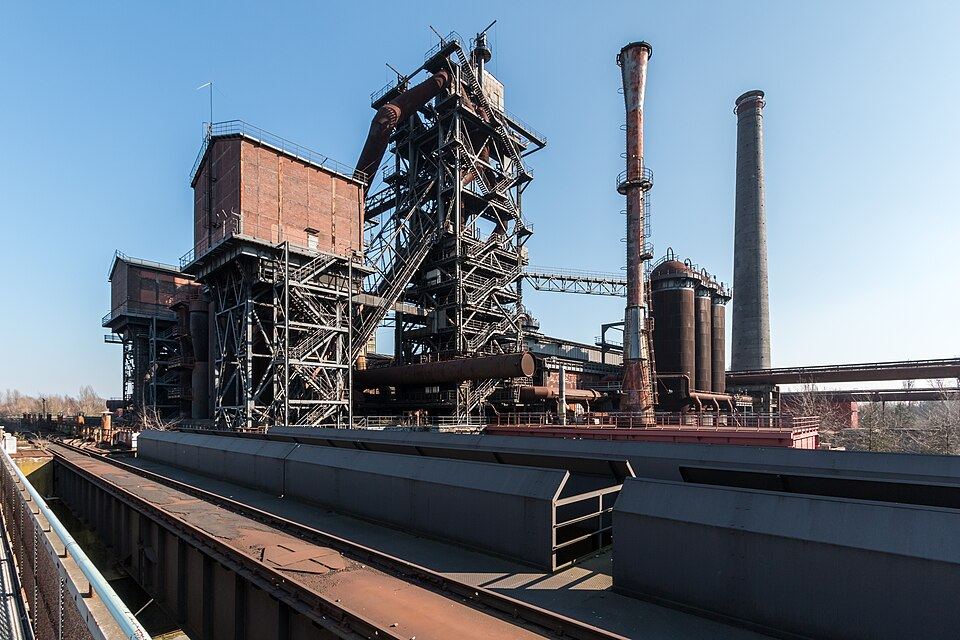
\includegraphics[width=0.6\linewidth]{images/book3/blast-furnace.jpg}

{\small فرن عالٍ محفوظ نُصبًا تذكاريًا (دويسبورغ-نورد، أُوقف سنة
1985): العمود الطويل مع حلقة أنابيب الهواء الساخن، ومخارج الغاز
في القمة. (صورة: ديتمار رابيش، CC~BY-SA~4.0، ويكيميديا كومنز.)}
\end{omfigure}

\section{طرق أخرى إلى الفلز}

\begin{definition}[التعدين الحراري والتعدين المائي]\label{def:b2:ellingham:metallurgy}
\emph{التعدين الحراري}\index{تعدين حراري} يستخلص الفلز عند درجة حرارة
مرتفعة، باختزال أكسيده في فرن. و\emph{التعدين المائي}\index{تعدين مائي}
يستخلصه من محلول مائي. ومراحلهما المعتادة هي
\emph{التحميص}\index{تحميص} (تسخين خام كبريتيدي في الهواء لتحويله إلى
أكسيد، \ce{2ZnS + 3O2 -> 2ZnO + 2SO2})، و\emph{الرشح}\index{رشح}
(إذابة مركّب الفلز، كثيرًا في حمض الكبريتيك، \ce{ZnO + 2H+ ->
Zn^2+ + H2O})، وتنقية المحلول، مثلًا
\emph{بالترسيب الإحلالي}\index{ترسيب إحلالي} (اختزال أيونات فلز أنبل
بمسحوق فلز أقل نبلًا، \ce{Cu^2+ + Zn -> Cu + Zn^2+})، ثم
استرجاع الفلز، كثيرًا بالتحليل الكهربائي.
\end{definition}

يفسّر المخطط تقاسم الأدوار. فالحديد والزنك والرصاص والقصدير تُستخلص
بالكربون في فرن. والألومنيوم، الذي يقع خطه أدنى بكثير من خط الكربون عند كل
درجة حرارة عملية، يُصنع بالتحليل الكهربائي لأكسيده المنصهر
(\cref{ch:b2:batteries-electrolysis})؛ والمغنيسيوم بالتحليل الكهربائي أو
بالاختزال بالسيليكون تحت التفريغ، الذي يزيل بخار المغنيسيوم؛
والتيتانيوم بتحويل الأكسيد إلى الكلوريد، \ce{TiO2 + 2Cl2 + C -> TiCl4 +
CO2} (\cref{exo:b2:reaction-free-energy:12})، ثم اختزال الكلوريد
بالمغنيسيوم (طريقة كرول). وأغلب زنك العالم يُصنع \omterm{def:b2:ellingham:metallurgy}{بالتحميص}،
\omterm{def:b2:ellingham:metallurgy}{والرشح}، والتحليل الكهربائي: فطريق \omterm{def:b2:ellingham:metallurgy}{التعدين المائي} يعطي فلزًا أنقى
ويتجنب التعامل مع بخار الزنك.

\begin{omfigure}
\begin{tikzpicture}[font=\small, >={Stealth}, box/.style={draw, thick, rounded corners=2pt, align=center, minimum height=0.9cm, fill=white, text width=2.3cm}]
  \node[box] (r) at (0,0) {\foreignlanguage{arabic}{تحميص}\\ \babelsublr{\ce{ZnS} $\to$ \ce{ZnO}}};
  \node[box] (l) at (3.2,0) {\foreignlanguage{arabic}{رشح}\\ \foreignlanguage{arabic}{في \ce{H2SO4}}};
  \node[box] (c) at (6.4,0) {\shortstack{\foreignlanguage{arabic}{تنقية}\\\foreignlanguage{arabic}{(ترسيب إحلالي)}}};
  \node[box] (e) at (9.6,0) {\foreignlanguage{arabic}{تحليل كهربائي}\\ \babelsublr{\ce{Zn^2+} $\to$ \ce{Zn}}};
  \draw[->, thick] (r) -- (l); \draw[->, thick] (l) -- (c); \draw[->, thick] (c) -- (e);
  \draw[->, thick, black!60] (r.north) -- ++(0,0.7) node[above] {\babelsublr{\ce{SO2} $\to$ \foreignlanguage{arabic}{حمض الكبريتيك}}};
  \draw[->, thick, omThm] (e.south) -- ++(0,-0.6) -| (l.south) node[pos=0.25, below] {حمض معاد};
  \draw[->, thick] (e.east) -- ++(0.8,0) node[right] {زنك};
\end{tikzpicture}

{\small طريق \omterm{def:b2:ellingham:metallurgy}{التعدين المائي} إلى الزنك. يُحوَّل ثنائي أكسيد الكبريت الصادر عن المحمصة
إلى حمض الكبريتيك اللازم \omterm{def:b2:ellingham:metallurgy}{للرشح}؛ ويُعاد إليه الحمض المتجدد عند
مصعد التحليل الكهربائي.}
\end{omfigure}

\section{تمارين}

\begin{exercise}[$\star$]\label{exo:b2:ellingham:1}
اكتب التفاعلات التي تمثلها خطوط أكسيد النحاس(I)، والألومينا، وأحادي أكسيد
الكربون، وثنائي أكسيد الكربون، كلًّا لمول واحد من \ce{O2}.
\end{exercise}

\begin{exercise}[$\star$]\label{exo:b2:ellingham:2}
انطلاقًا من قيم كوداتا المرجعية ($\Delta_f H^\circ(\ce{ZnO}) = \qty{-350.46}{kJ/mol}$،
و$S^\circ$: \ce{ZnO} 43.65، \ce{Zn} 41.63، \ce{O2} \qty{205.15}{J/(K.mol)})،
اكتب $\Delta_r G^\circ(T)$ للتفاعل \ce{2Zn + O2 -> 2ZnO} من أجل زنك صلب.
\end{exercise}

\begin{exercise}[$\star$]\label{exo:b2:ellingham:3}
مستعملًا المخطط، اذكر الفلزات التي تستطيع اختزال أكسيد الكروم(III) عند
\qty{1500}{K}، والفلزات التي لا تستطيع.
\end{exercise}

\begin{exercise}[$\star$]\label{exo:b2:ellingham:4}
فسّر إشارة ميل كل خط من خطوط الكربون الثلاثة.
\end{exercise}

\begin{exercise}[$\star\star$]\label{exo:b2:ellingham:5}
احسب \omterm{def:b2:ellingham:oxygen-pressure}{ضغط الأكسجين التوازني} لأكسيد الزئبق(II) عند \qty{600}{K}
(الزئبق سائل، $\Delta_r H^\circ = \qty{-181.6}{kJ}$، $\Delta_r S^\circ =
\qty{-216.5}{J/K}$ لكل مول من \ce{O2}). هل يتأكسد الزئبق في الهواء عند تلك
الدرجة؟
\end{exercise}

\begin{exercise}[$\star\star$]\label{exo:b2:ellingham:6}
احسب $\Delta_r G^\circ$ عند \qty{298}{K} لتفاعل الثرميت، \ce{Fe2O3 +
2Al -> Al2O3 + 2Fe}، علمًا أن $\Delta_f G^\circ = \qty{-743.5}{kJ/mol}$ للمركب
\ce{Fe2O3} و\qty{-1582.3}{kJ/mol} للمركب \ce{Al2O3}، وبيّن لماذا لا يبدأ التفاعل،
مع أنه شديد الطرد للطاقة، في درجة حرارة الغرفة.
% ledger: janafG:Fe2O3.298, janafG:Al2O3.298
\end{exercise}

\begin{exercise}[$\star\star$]\label{exo:b2:ellingham:7}
جِد على المخطط درجة الحرارة التي يختزل الكربون فوقها أكسيد الحديد(II)
إلى حديد مع تكوين أحادي أكسيد الكربون، واكتب التفاعل.
\end{exercise}

\begin{exercise}[$\star\star$]\label{exo:b2:ellingham:8}
عند \qty{1100}{K}، $\Delta_f G^\circ(\ce{CO}) = \qty{-209.1}{kJ/mol}$ 
و$\Delta_f G^\circ(\ce{CO2}) = \qty{-396.0}{kJ/mol}$. احسب $K^\circ$ \omterm{def:b2:ellingham:boudouard}{لتوازن
بودوار} والكسر المولي لأحادي أكسيد الكربون فوق الكربون عند
\qty{1}{bar}. ماذا يحدث للغاز، على تماس مع السخام أو الحديد، حين
يُبرَّد إلى \qty{700}{K}؟
% ledger: janafG:CO.1100, janafG:CO2.1100
\end{exercise}

\begin{exercise}[$\star\star$]\label{exo:b2:ellingham:9}
يُستعمل الهيدروجين أحيانًا لاختزال أكسيد التنغستن. مستعملًا خط الماء،
فسّر لماذا يكون الهيدروجين مختزلًا أفضل من أحادي أكسيد الكربون عند درجة حرارة
مرتفعة لكنه أسوأ منه عند درجة حرارة منخفضة.
\end{exercise}

\begin{exercise}[$\star\star\star$]\label{exo:b2:ellingham:10}
يمكن اختزال أكسيد المغنيسيوم بالسيليكون، \ce{2MgO + Si -> SiO2 + 2Mg}، مع أن
خط السيليكا يقع فوق خط أكسيد المغنيسيوم عند كل درجات حرارة
المخطط. عند \qty{1500}{K} يكون المغنيسيوم غازًا وتعطي الجداول، لكل مول من
\ce{O2}، \qty{-845.5}{kJ} لأكسيد المغنيسيوم و\qty{-643.7}{kJ} للسيليكا.
احسب $\Delta_r G^\circ$ للاختزال، ثم ضغط بخار المغنيسيوم
الذي يجري التفاعل تحته في الاتجاه المباشر. كيف يستفيد فرن التفريغ من ذلك؟
% ledger: janafG:MgO.1500, janafG:SiO2.1500
\end{exercise}

\begin{exercise}[$\star\star\star$]\label{exo:b2:ellingham:11}
احسب \omterm{def:b2:equilibrium-shifts:variance}{تغايرية} النظام \ce{FeO(s)}، \ce{Fe(s)}، \ce{CO(g)}،
\ce{CO2(g)} في توازن. ماذا يعني ذلك للغاز الخارج من الجزء العلوي
من الفرن العالي؟
\end{exercise}

\begin{exercise}[$\star\star\star$]\label{exo:b2:ellingham:12}
يُنقّى النحاس من محلول رشحه \omterm{def:b2:ellingham:metallurgy}{بالترسيب الإحلالي} بخردة الحديد.
مستعملًا الجهود المعيارية الواردة في مجلد السنة الأولى ($E^\circ(\ce{Cu^2+}/\ce{Cu})
= \qty{0.34}{V}$، $E^\circ(\ce{Fe^2+}/\ce{Fe}) = \qty{-0.41}{V}$)، احسب
ثابت التوازن للتفاعل \ce{Cu^2+ + Fe -> Cu + Fe^2+} والتركيز
المتبقي لأيونات النحاس حين يحوي المحلول \qty{1.0}{mol/L} من
\ce{Fe^2+}.
\end{exercise}

\section{مسألة: الزنك بالنار}

\begin{problem}[{مسألة نهاية الأسبوع --- خطا إلينغهام لأكسيد الزنك
ولأحادي أكسيد الكربون، ودرجة الحرارة التي يختزل عندها الكربون أكسيد الزنك،
وتغايرية الفرن، وتكثف بخار الزنك}]
\label{pb:b2:ellingham:1}
قبل التحليل الكهربائي، كان الزنك يُصنع بتسخين أكسيده مع الكربون في
معوجات من الطين. المعطيات (كوداتا، وجدول جاناف للزنك): $\Delta_f H^\circ(\ce{ZnO})
= \qty{-350.46}{kJ/mol}$؛ $S^\circ$ (\unit{J/(K.mol)}): \ce{ZnO} 43.65، \ce{Zn}
41.63، \ce{O2} 205.15؛ ينصهر الزنك عند \qty{692.7}{K} ($\Delta_{\text{انصهار}}H =
\qty{7.32}{kJ/mol}$) ويغلي عند \qty{1180.2}{K} تحت \qty{1}{bar}
($\Delta_{\text{تبخر}}H = \qty{115.3}{kJ/mol}$). ومن أجل \ce{2C + O2 -> 2CO}، تعطي
الجداول $\Delta_r G^\circ = \qty{-418.2}{kJ}$ عند \qty{1100}{K} 
و\qty{-453.0}{kJ} عند \qty{1300}{K}.
% ledger: dfh:ZnO_cr, s0:ZnO_cr, s0:Zn_cr, s0:O2_g, hT:Zn_cr.692, hT:Zn_l.692, hT:Zn_l.1180, hT:Zn_g.1180, dfh:Zn_g, janafG:CO.1100, janafG:CO.1300

\medskip
\noindent\textbf{الجزء الأول --- خط أكسيد الزنك.}
\begin{enumerate}
  \item احسب $\Delta_r H^\circ$ و$\Delta_r S^\circ$ للتفاعل \ce{2Zn(s) + O2 ->
        2ZnO} عند \qty{298}{K}.
  \item اكتب $\Delta_r G^\circ(T)$ تحت نقطة الانصهار.
  \item احسب إنتروبيا انصهار الزنك وإنتروبيا تبخره.
  \item اكتب $\Delta_r G^\circ(T)$ بين نقطتي الانصهار والغليان.
  \item اكتبها فوق نقطة الغليان.
  \item احسب الميول الثلاثة وفسّر لماذا يكون الأخير أشد حدة بكثير.
  \item تحقق من أن العبارات الثلاث تتفق عند درجات حرارة التحول.
\end{enumerate}

\medskip
\noindent\textbf{الجزء الثاني --- خط الكربون.}
\begin{enumerate}[resume]
  \item انطلاقًا من القيمتين المجدولتين، اكتب خط \ce{2C + O2 -> 2CO} على
        الصورة $a + bT$ بين \qty{1100}{K} و\qty{1300}{K}.
  \item استنتج $\Delta_r S^\circ$ له وفسّر إشارته.
  \item اكتب الاختزال \ce{ZnO + C -> Zn(g) + CO} و$\Delta_r
        G^\circ(T)$ له على أنه فرق الخطين (لكل مول من \ce{O2}).
  \item جِد درجة الحرارة التي يتقاطع عندها الخطان.
  \item لماذا يهم أن تكون هذه الدرجة فوق نقطة غليان
        الزنك؟
\end{enumerate}

\medskip
\noindent\textbf{الجزء الثالث --- المعوجة.}
\begin{enumerate}[resume]
  \item احسب \omterm{def:b2:equilibrium-shifts:variance}{تغايرية} النظام \ce{ZnO(s)}، \ce{C(s)}، \ce{Zn(g)}،
        \ce{CO(g)}، والزنك وأحادي أكسيد الكربون لا يتكونان إلا بالاختزال.
  \item في معوجة عند \qty{1300}{K} تحت \qty{1}{bar}، ما الضغطان الجزئيان
        للزنك ولأحادي أكسيد الكربون إذا كان التفاعل تامًا؟
  \item احسب $\Delta_r G^\circ$ للاختزال عند \qty{1300}{K} والثابت
        $K^\circ$ الموافق.
  \item فسّر لماذا تُشغَّل المعوجة فوق درجة حرارة التقاطع بقليل
        لا فوقها بكثير.
\end{enumerate}

\medskip
\noindent\textbf{الجزء الرابع --- المكثِّف.}
\begin{enumerate}[resume]
  \item يُقاد البخار إلى مكثِّف أبرد. اكتب التفاعل الذي قد يُعاد به
        تأكسد بخار الزنك بثنائي أكسيد الكربون.
  \item مستعملًا المخطط، فسّر لماذا يجب إبقاء الغاز خاليًا من ثنائي
        أكسيد الكربون.
  \item لماذا يجب تكثيف الزنك بسرعة لا ببطء؟
  \item احسب كتلة الكربون اللازمة لكل طن من الزنك، مع أخذ
        الاختزال كما هو مكتوب.
  \item احسب الحرارة الممتصة لكل طن من الزنك بالاختزال عند نحو
        \qty{1300}{K} (خذ $\Delta_r H^\circ$ من عبارات الجزأين الأول
        والثاني).
  \item اذكر درجة الحرارة التي يختزل الكربون فوقها أكسيد الزنك في
        الشروط القياسية.
\end{enumerate}
\end{problem}
